%----------------------------------------------------------------------------
%
% 
% 
%
%----------------------------------------------------------------------------
%----------------------------------------------------------------------------
%----------------------------------------------------------------------------

\ProvidesFile{proposal.tex}
\documentclass[cameraready]{acmsiggraph-awb}
\usepackage[scaled=.92]{helvet}
\usepackage{times}
\usepackage{algorithm}
\usepackage{algorithmic}

\usepackage[pdftex]{graphicx} \pdfcompresslevel=9

\usepackage{parskip}

\usepackage[labelfont=bf,textfont=it]{caption}

\usepackage{amsmath}
\usepackage{amssymb}
\usepackage{wasysym}
\usepackage{bm}
\usepackage{cite}

\usepackage{enumerate}

\usepackage{url}

% For backwards compatibility to old LaTeX type font selection.
% Uncomment if your document adheres to LaTeX2e recommendations.
\let\rm=\rmfamily    \let\sf=\sffamily    \let\tt=\ttfamily
\let\it=\itshape     \let\sl=\slshape     \let\sc=\scshape
\let\bf=\bfseries

% end of prologue
\usepackage[%
 breaklinks,
 letterpaper,
 bookmarks,
 bookmarksnumbered,
 colorlinks,
 linkcolor={black},
 citecolor={black},
 pdfpagemode={None},
]{hyperref}
\setlength\paperwidth{8.5in}  % Override any random settings...
\setlength\paperheight{11in}

\DeclareMathOperator*{\argmin}{\arg\!\min}


\newcommand{\etal}{et al.}
\newcommand{\hidecomment}[1]{}
\newcommand{\Mueller}{M\"{u}ller\ }
\newcommand{\Bez}{B\'{e}zier\ }
\newcommand{\BM}[1]{\B{#1}}
%\newcommand{\B}[1]{\mbox{\boldmath$#1$}}
%\newcommand{\B}[1]{\textbf{\textit{#1}}}
\newcommand{\B}[1]{\mathit{\mathbf{#1}}}
%\newcommand{\B}[1]{\boldsymbol{#1}}
\newcommand{\Per}{\%}
\newcommand{\Unit}[1]{{\mbox{$\,\mathrm{#1}$}}}
\newcommand{\Snit}[1]{{\mbox{\small$\mathrm{#1}$}}}
\newcommand{\Tr}[1]{\mathrm{Tr}\left(#1\right)}
\newcommand{\Hz}{\Unit{Hz}}
\newcommand{\MHz}{\Unit{MHz}}
\newcommand{\GHz}{\Unit{GHz}}
\newcommand{\Sec}{\Unit{sec}}
\newcommand{\SPF}{\Unit{sec/frame}}
\newcommand{\Min}{\Unit{min}}
\newcommand{\Max}{\Unit{max}}
\newcommand{\M}{\Unit{m}}
\newcommand{\Nab}{\B{\nabla}}
\newcommand{\TP}{^\mathsf{T}}

\newcommand{\Dist}{\mbox{dist}}

\newcommand{\figureTopBot}[1]{
  \begin{figure}[!tb]{\sloppy #1}\end{figure}
}

\newcommand{\figureTop}[1]{
  \begin{figure}[!t]{\sloppy #1}\end{figure}
}
 
\newcommand{\figureBot}[1]{
  \begin{figure}[!b]{\sloppy #1}\end{figure}
}

\newcommand{\figureWideTop}[1]{
  \begin{figure*}[!t]{\sloppy #1}\end{figure*}
}

\newcommand{\eqAlgn}{\!\!&\!\!}

\newcommand{\Eref}[1]{Equation~(\ref{#1})}
\newcommand{\Erefs}[2]{Equations~(\ref{#1}) and (\ref{#2})}
\newcommand{\eref}[1]{Equation~(\ref{#1})}
\newcommand{\erefs}[2]{Equations~(\ref{#1}) and (\ref{#2})}
\newcommand{\Sref}[1]{Section~\ref{#1}}
\newcommand{\sref}[1]{Section~\ref{#1}}
\newcommand{\fref}[1]{Figure~\ref{#1}}
\newcommand{\frefAND}[2]{Figures~\ref{#1} and~\ref{#2}}
\newcommand{\frefs}[2]{Figures~\ref{#1} and~\ref{#2}}
\newcommand{\frefss}[3]{Figures~\ref{#1}, \ref{#2}, and~\ref{#3}}
\newcommand{\Fref}[1]{Figure~\ref{#1}}
\newcommand{\Frefs}[2]{Figures~\ref{#1} and~\ref{#2}}
\newcommand{\Frefss}[3]{Figures~\ref{#1}, \ref{#2}, and~\ref{#3}}
\newcommand{\tref}[1]{Table~\ref{#1}}

\renewcommand{\labelenumi}{\arabic{enumi}.}
\renewcommand{\labelenumii}{\alph{enumii}.}
\renewcommand{\labelenumiii}{\roman{enumiii}.}

\newenvironment{algstep}{%
  \begin{enumerate}%
    \setlength{\itemsep}{0in}%
    \setlength{\partopsep}{0in}%
    \setlength{\topsep}{0in}%
}{\end{enumerate}}





\onlineid{papers\_0632}
\newcommand{\theTitle}{GPU Accelerated Point-Based Elastoplastic Solid Simulation}

\title{\theTitle}

\author{
	Ben Jones \and Kyle Hansen}

\newcommand{\theKeywords}{%
  viscoelastic materials, point-based animation, natural phenomena, physics-based animation.%
}


\begin{document}

\teaser{\begin{centering}
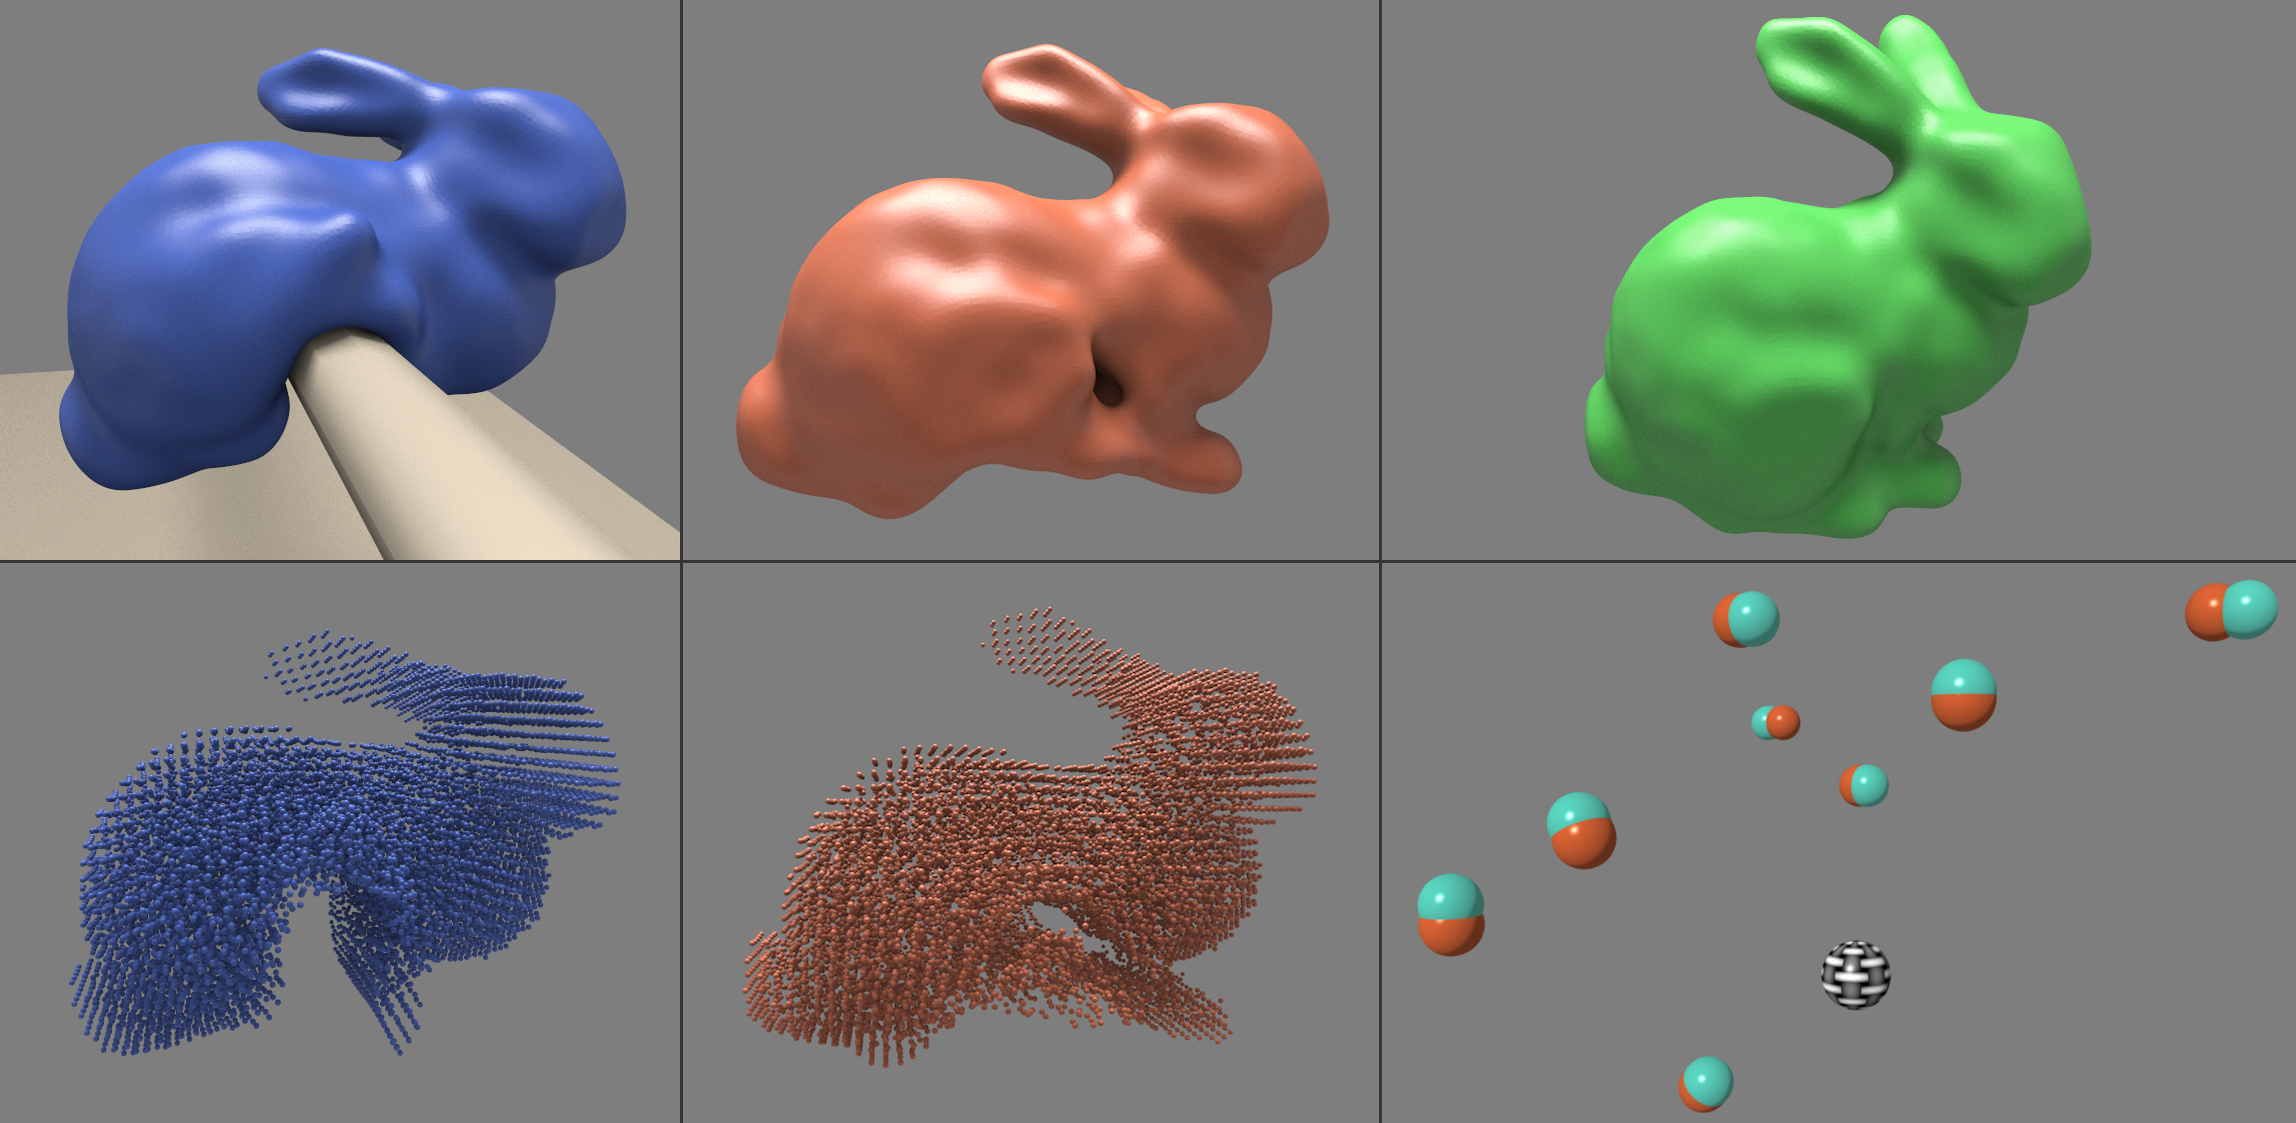
\includegraphics[width=6.1in]{Figures/teaser.png}
\caption{Sample frames from a sequential, point-based elastoplastic simulator, which is being accelerated with a GPU implementation for this project.}
\label{fig:teaser}
\end{centering}
}

\maketitle




\section{Team members}

\begin{itemize}

\item Ben Jones: Part of the team that implemented the sequential version of this algorithm, working with Adam Bargteil on graphics simulation research.
Will be focusing on the core algorithm parallelization.

\item Kyle Hansen: Computing Masters Student in the Graphics and Visualization Track.  
2+ years of real world programming experience as an electronics engineer.  
Hobby game programmer.  
Will be primarily concerned with the real time openGL rendering of simulation results and nearest neighbor calculations.

\end{itemize}

\section{Problem Description}

Simulating deformable solids is important for creating visual effects.  To generate compelling effects, we need to be able to handle materials across the entire spectrum from highly elastic, to totally plastic.  Using finite element methods with volumetric meshes (often tetrahedral) is a common approach, but large plastic deformation creates poorly conditioned tetrahedra.  To handle this, complicated volumetric remeshing is necessary to maintain stability and accuracy.  Recently, several point based methods have been proposed to avoid these expensive/complex operations.  However, these methods often support only one end of the spectrum, elastic or plastic materials, but not both  \cite{Mueller:2004:PBA}, \cite{Gerszewski:2009:APB}.  Recently, Jones et al. \cite{us} proposed a new point based technique that handles materials across the range between elastic and plastic.  The goal of our project is to improve performance of their method by performing as much computation as possible on the GPU.  

\section{Algorithm Description}

During elastoplastic simulation, deformation is computed by comparing the current deformed configuration of point samples with their reference configuration.  This deformation, along with material properties, is used compute elastic forces and plastic deformation of the reference configuration.  This is shown schematically in Figure \ref{fig:defGrad}.
\begin{figure}
\begin{centering}
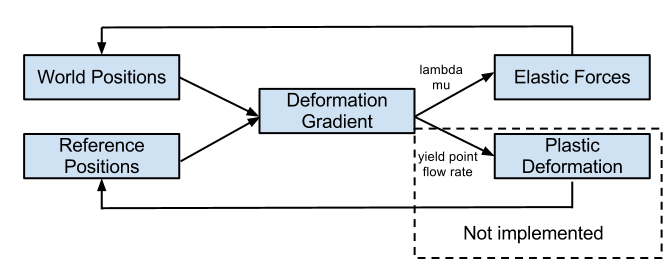
\includegraphics[width = 5in]{Figures/algSchematic.png}
\caption{The difference between world and reference configurations defines the deformation gradient, which, along with material parameters, defines elastic forces and plastic deformation.}
\label{fig:defGrad}
\end{centering}
\end{figure}


During the simulation, we maintain the objects world configuration, a set of nearest neighbors for each particle, and least squares fit of the global reference configuration.  At each simulation time step, we perform the following steps:
\begin{itemize}

\item compute deformation gradient, per particle
\begin{itemize}
\item factor gradient into elastic and plastic components
\item apply elastic and body (gravity) forces
\item apply plastic deformation to vectors to all neighbors of a particle*
\end{itemize}
\item integrate elastic forces
\begin{itemize}
\item perform explicit integration step of elastic and body forces
\item perform implicit damping force solve* 
\end{itemize}
\item compute new world reference configuration* 
\item compute per particle local error in global reference configuration* 
\item update particle neighborhoods 
\item resolve obstacle collisions
\item render current simulation frame (using openGL)**
\item write particle positions to file*
\end{itemize}

* Not yet included in the CUDA implementation.

** Unique to the CUDA implementation.

For more details please refer to \cite{us}.
It should be noted that the above steps outline the complete simulation algorithm, which has not all been implemented for this particular project.
For this project, we have only considered the elastic and body forces while also accelerating the K nearest neighbor (KNN) calculations and incorporating OpenGL to render the results as they are calculated.
The primary goal for this project is to illustrate the potential acceleration that could be acheived by incorporating CUDA parallelization into the simulation.


\section{Suitability for GPU implementation}

Since the simulation is particle based, there is no explicit connectivity in the object, and hence, few data dependencies.  
Most steps involve computing 3x3 matrices based on local information, or information from neighbor particles.  
Within these steps, very little synchronization is required, since most writes are to a particle's own data. 
Therefore, most of the algorithm is inherently parallel, and we expect to see speedups by performing operations on the GPU.  

The two global solves involve solving sparse symmetric positive definite matrices using the conjugate gradient algorithm.  Each iteration requires a matrix multiply and a few dot products.  As stated in class, these operations don't perform particularly well on a GPU, but easily outperform CPU implementations.  Rough profiling of the sequential implementation revealed that these solves take the majority of the computation time, in some cases as much as 90\%.   Hence any speedup by performing these computations on the GPU will make a significant difference in overall runtime.  Additionally, the matrices do not need to be stored explicitly; the matrix vector multiplication operation can be implemented as a loop over particles and their neighbors, resulting in predictable memory accesses and little synchronization.  

Researchers have studied solving the K Nearest Neighbors problem using the GPU.   The work of \cite{Garcia_2008_CVGPU} provides a CUDA implementation that provides speedup over sequential implementations.  Even if a sequential implementation is used for finding neighbors, it is performed infrequently (every 10 time steps), so copy overhead would not be a dominating cost.  

By performing the computation on the GPU, we can share data with OpenGL in a vertex buffer object (VBO), so that no copying is necessary between CPU and GPU except at the first frame of simulation.  


\section{Mapping to the GPU}

Because particles behave almost completely independently, we chose to map each particle to a single CUDA thread.  Most steps in the algorithm require only reads from neighboring particle positional data and computation on 3 by 3 matrices.  Each particle tracks position and velocity in world space, reference position, forces, and indices of neighbor particles.  The position data is shared with OpenGL using a VBO.  A schematic representation of the mapping is shown in Figure \ref{fig:mapping}.


\begin{figure}
\begin{centering}
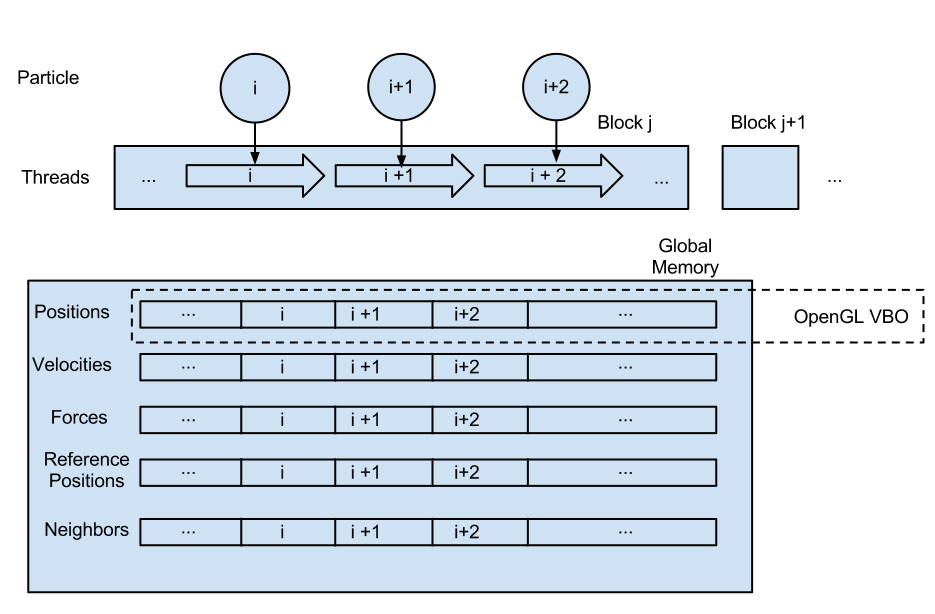
\includegraphics[width = 5in]{Figures/threadDecomp.png}
\caption{Decomposition of the algorithm onto the GPU.}
\label{fig:mapping}
\end{centering}
\end{figure}

There are several points in the algorithm that require global synchronization.  
For example, a particle needs to wait for all neighboring particles to apply forces to it before integrating in time.  
To handle this, we used several separate CUDA kernels.  
This causes more scheduling overhead, but since we are not copying data, this will likely not have a significant performance impact for large simulations.  
Figure \ref{fig:kernelDivision} illustrates this division.  
Additionally, atomic addition is required to avoid race conditions when calculating the forces between all neighboring particles.

\begin{figure}
\begin{centering}
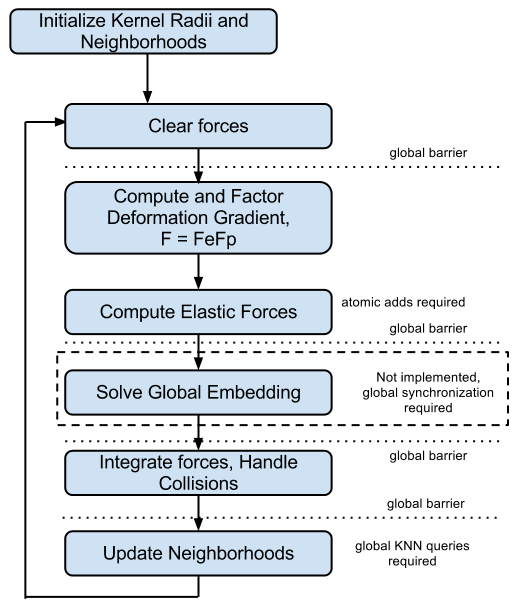
\includegraphics[width = 3in]{Figures/AlgorithmFlowchart.png}
\caption{Overview or required synchronization.}
\label{fig:kernelDivision}
\end{centering}
\end{figure}

\section{Rendering with OpenGL}

A major advantage of using CUDA for this simulation is that results can be rendered efficiently as they are calculated, since the data is already stored on the GPU.
We displayed the results by swapping a data buffer back and forth between OpenGL and CUDA.  
CUDA includes functions specifically for this type of interaction.  
The buffer is initially created as an OpenGL VBO, but during CUDA kernel calls, it is unmapped for OpenGL while its data is manipulated by the CUDA code.
At the completion of the kernel function, the buffer is mapped back to OpenGL where it is rendered.
This buffer contains the position data for the particles in the simulation as 4-tuple float values, corresponding to the X, Y, Z, and W homogenous coordinates.
This is represented using a float4 data type in CUDA.
The positions are rendered simply as points in our code, though if more impressive graphics are desired, shaders could be added to improve the final appearence as is done in one of the CUDA SDK examples.

Incorporating OpenGL into a CUDA program introduces a fair amount of additional overhead and has a significant impact on the overall structure and organization of the code.
Once all the initialization has been taken care of for both CUDA and OpenGL, the program enters into the main animation loop for OpenGL.  
While in this loop, it uses several callback functions to handle input and output.
We made the CUDA kernel calls from within the ``display`` callback function.
This way, the display is updated as soon as new results are calculated.  
The downside of this organization is that as the kernel execution time increases for larger simulations, it causes the display function to take longer, which results in a sluggish program response to user input.


\begin{figure}
\begin{centering}
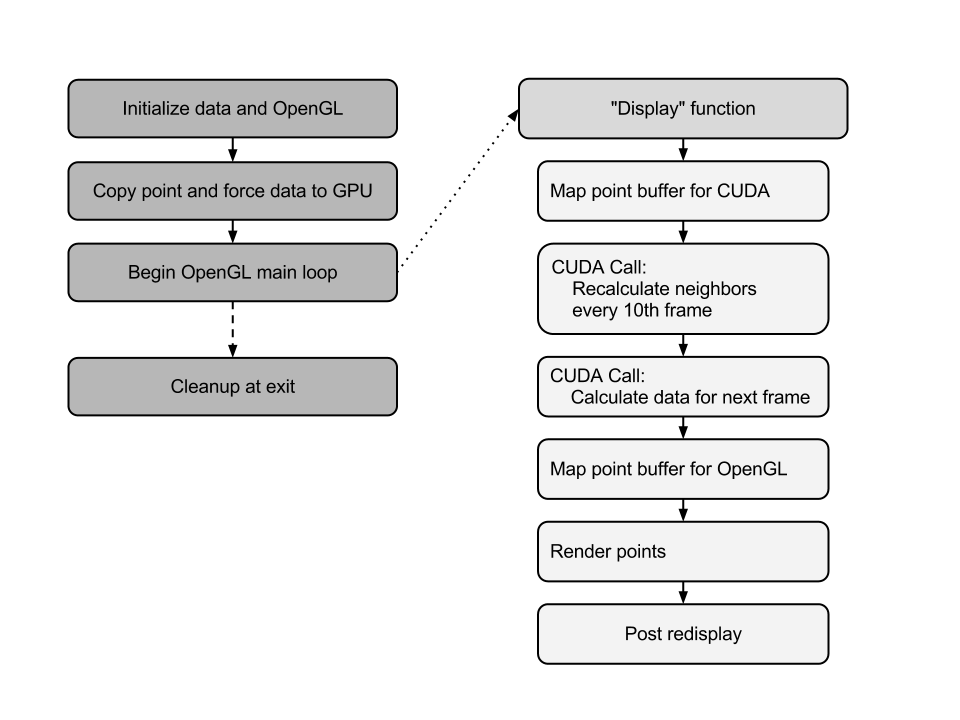
\includegraphics[width = 5in]{Figures/openglFlowchart.png}
\caption{Overview of control flow between OpenGL and CUDA.}
\label{fig:kernelDivision}
\end{centering}
\end{figure}

\section{Calculating Nearest Neighbors}

The calculation of nearest neighbors among particles is easily the most expensive operation in this simulation.  
Luckily, neighborhoods tend to change little from one frame to the next, so recalculating neighbors every frame would be overkill.
Instead, nearest neighbors are calculated for every 10th frame, and those results are reused until the next time they are updated.
Even so, the KNN calculations tend to have the largest impact on overall execution time.
As an illustration, for 512 particles and 32 neighbors, a typical frame with no KNN calculations took around 5ms to update while those frames updating the neighborhoods tended to take over 100ms.
For a larger simulation, with 32768 particles and 32 neighbors, KNN calculations took over 2 full seconds while frames between neighborhood updates required less than 25ms.

The KNN calculations are an obvious target for optimization.
For this project, we deferred to the work of \cite{Garcia_2008_CVGPU} who provided a CUDA implementation for calculating K nearest neighbors.
They basically use CUDA to parallelize the brute force approach for calculating KNN.  
Their claim is that the brute force method is more suited to parallel execution than alternative methods.
They make use of texture memory for non-coalesced memory access during the calculations, and they use an insertion sort to order distances since it tends to be more efficient when only a relatively small number of the top entries are desired.
Their implementation of KNN was definitely faster than the brute force method of comparing all points, which we used while getting the KNN code to work, though this was still the most time consuming piece of our simulation code.

Because we used their code with minimal modification, there were a few missed opportunities for context-specific optimization.  
There was also overhead for copying data between the host and device, since the KNN function expected input at the host level and that was also where it saved the final results.
Additionally, the KNN function expected a different format for the data than what we needed for OpenGL to understand it, so an extra function was written to convert the data between formats.
These factors reduced the efficiency of the KNN calculations somewhat, but they were negligible compared to the total time of executing the KNN function itself, which took about 1000 times longer than copying or converting the values.

Given more time to work on it, the most likely opportunity here for a significant performance improvement would be to re-implement the KNN function so that it makes use of the known positions from previous neighborhood calculations since, as has been mentioned before, the neighborhoods are unlikely to change much over a short time period.
That could be an entire project in itself, however.

\section{Results}

We tested our simulator by dropping an evenly sampled cube onto flat ground.  Selected frames from one simulation are shown in Figure \ref{fig:combined}.  
\begin{figure}
\begin{centering}
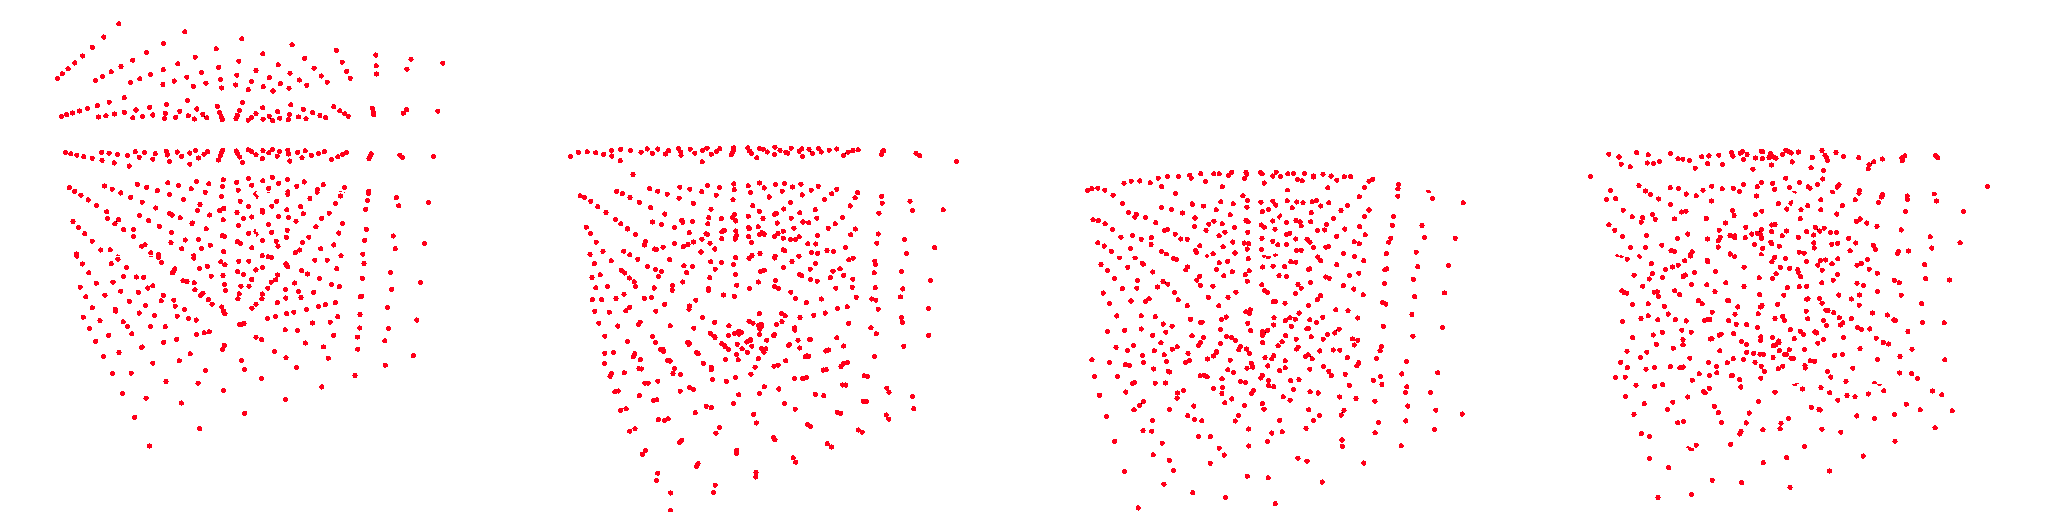
\includegraphics[width = 5in]{Figures/combined.png}
\caption{Example simulation of box being dropped on flat ground.}
\label{fig:combined}
\end{centering}
\end{figure}


We compared our results to a sequential implementation in order to determine the speedup of our parallel algorithm.  Sequential computations were performed on a single core of a 2.4GHz Intel Core I-5 processor.  Figure \ref{fig:scaling1} and Table \ref{tab:scaling1} show how our method scales with the number of particles, and the number of neighbors per particle.  Especially with a large number of particles, the CUDA implementation is significantly faster than the sequential implementation.


\begin{figure}
\begin{centering}
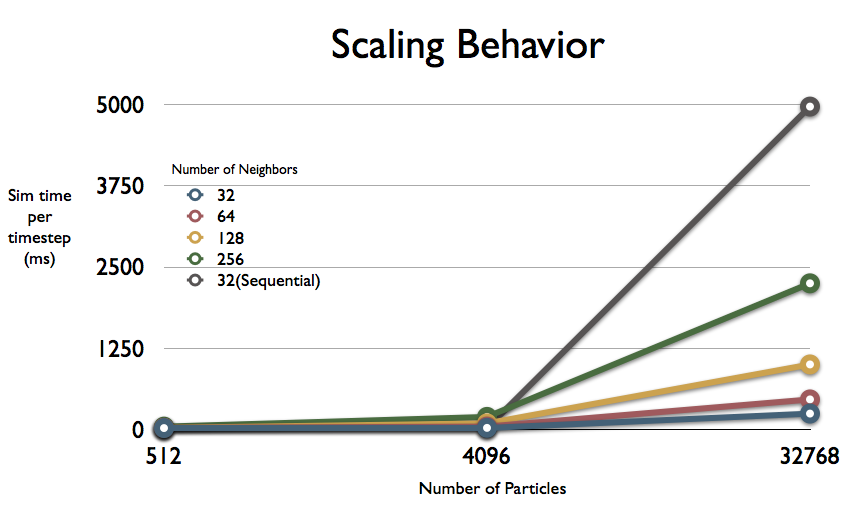
\includegraphics[width = 5in]{Figures/charts_001.png}
\caption{Scaling behavior of our implementation.  It significantly outperforms the sequential code for large examples.}
\label{fig:scaling1}
\end{centering}
\end{figure}

\begin{table}[htdp]
\caption{Runtimes per timestep (ms)}
\begin{center}
\begin{tabular}{c|ccc}
Number of neighbors& \multicolumn{3}{c}{Number of particles} \\
&512&   4096&   32768 \\ \hline

32& 22&	25&	245 \\
64& 25&	45&	463 \\
128& 26	&95	&1001 \\
256& 44	&194&	2249 \\
32(sequential)& 23	&26	&4968  \\
\end{tabular}
\end{center}
\label{tab:scaling1}
\end{table}%


We also analyzed how the KNN queries contributed to our runtime.  Figure \ref{fig:scaling2} and Table \ref{tab:scaling2} show that the KNN queries are a significant bottleneck in the implementation, as shown by the huge difference between average and worst case timings.  


\begin{figure}
\begin{centering}
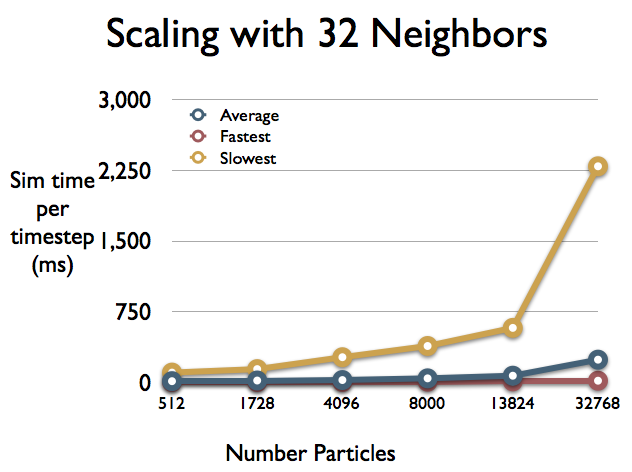
\includegraphics[width = 5in]{Figures/charts_002.png}
\caption{KNN query times are the bottleneck in our implementation (average vs slowest frames).}
\label{fig:scaling2}
\end{centering}
\end{figure}


\begin{table}[htdp]
\caption{Runtimes per timestep, 32 neighbors (ms)}
\begin{center}
\begin{tabular}{ccccccc}
& \multicolumn{6}{c}{Number of particles} \\
& 512 & 1728 & 4096 & 8000 & 13824 & 32768 \\ \hline
Average &14	&21	&26	&44	&72	&242 \\
Fastest & 5&	5&	6	&9	&12	&19 \\
Slowest & 105&	142	&268	&387	&579&	2292\\
\end{tabular}
\end{center}
\label{tab:scaling2}
\end{table}%

\section{Conclusions}

As expected, a CUDA implementation provided significant speedup over the sequential implementation of the simulation algorithm, especially for large problem sizes.  The computation required for each particle was enough to hide data latency, and keep the processing cores busy.  The KNN algorithm we used performed poorly compared to the KD-tree based approach used in the sequential implementation.  Investigating this further is a possible direction of future work.

Due to time constraints, we were not able to implement implicit integration or plastic deformation, but we are confident that both could be implemented efficiently with CUDA.  Due to the structure of the spare matrix systems being solved, we could achieve large speedups without significant fine-grained synchronization

Another direction of future work is taking more advantage of the memory hierarchy by copying data from nearby particles to shared memory.  This would require a block decomposition based on particle proximity, but could potentially lead to large speedups.  




%\section{Intellectual Challenges}
%
%We expect the biggest challenges to come from solving the sparse matrices.
%These will be large matrices and care will need to be taken to break them up effectively for parallel computation.
%That much is relatively straightforward and similar to previous assignments, but it will be further complicated by the use of sparse matrix methods.
%
%Aside from that, much of the simulation parallelization should simply involve converting loops into threaded CUDA functions, 
%although atomic operations or other synchronization methods may be necessary when calculating interactions between neighboring particles.
%
%Additionally, there may be some challenges in implementing the OpenGL rendering of the simulation.  
%Such difficulties will be due more to unfamiliarity with the process and libraries rather than it being theoretically difficult, 
%since CUDA already has functions that provide the ability to coordinate with OpenGL for rendering purposes.
%
%\begin{CRcatlist}
  %\CRcat{I.3.7}{Computer Graphics}{Three-Dimensional Graphics and Realism}{Animation};
  %\CRcat{I.6.8}{Simulation and Modeling}{Types of Simulation}{Animation}.
%\end{CRcatlist}

%\keywordlist


%----------------------------------------------------------------------------
%----------------------------------------------------------------------------




%\let\ORIGCaption\caption
%\renewcommand{\caption}[1]{\vspace{-0.025in}\ORIGCaption{#1}}

%----------------------------------------------------------------------------
%----------------------------------------------------------------------------


\bibliographystyle{acmsiggraph-awb}
\bibliography{elastoplasticCuda}

\end{document}

